%-----------------------------------------------------------------------
% Functional Programming 4
% John O'Donnell, Wim Vanderbauwhede
% University of Glasgow
%-----------------------------------------------------------------------

\documentclass{beamer}
\usepackage{jtodlecseriesFP4}
%include polycode.fmt
%format alpha = "\alpha"
%format ~> = "\leadsto "

% Identify this presentation
\SetPresentationTitle
  {Program Structure}
  {Program Structure}
\SetPresentationNumber
  {8}
\SetPresentationDate
  {Week 4-2}
  {Week 4-2}

%-----------------------------------------------------------------------
% Beginning

\begin{document}

\begin{frame}[fragile]
  \PresentationTitleSlide
\end{frame}

\begin{frame}[fragile]
  \frametitle{Topics}
  \tableofcontents
\end{frame}
%-----------------------------------------------------------------------
\begin{frame}[fragile]
\begin{center}
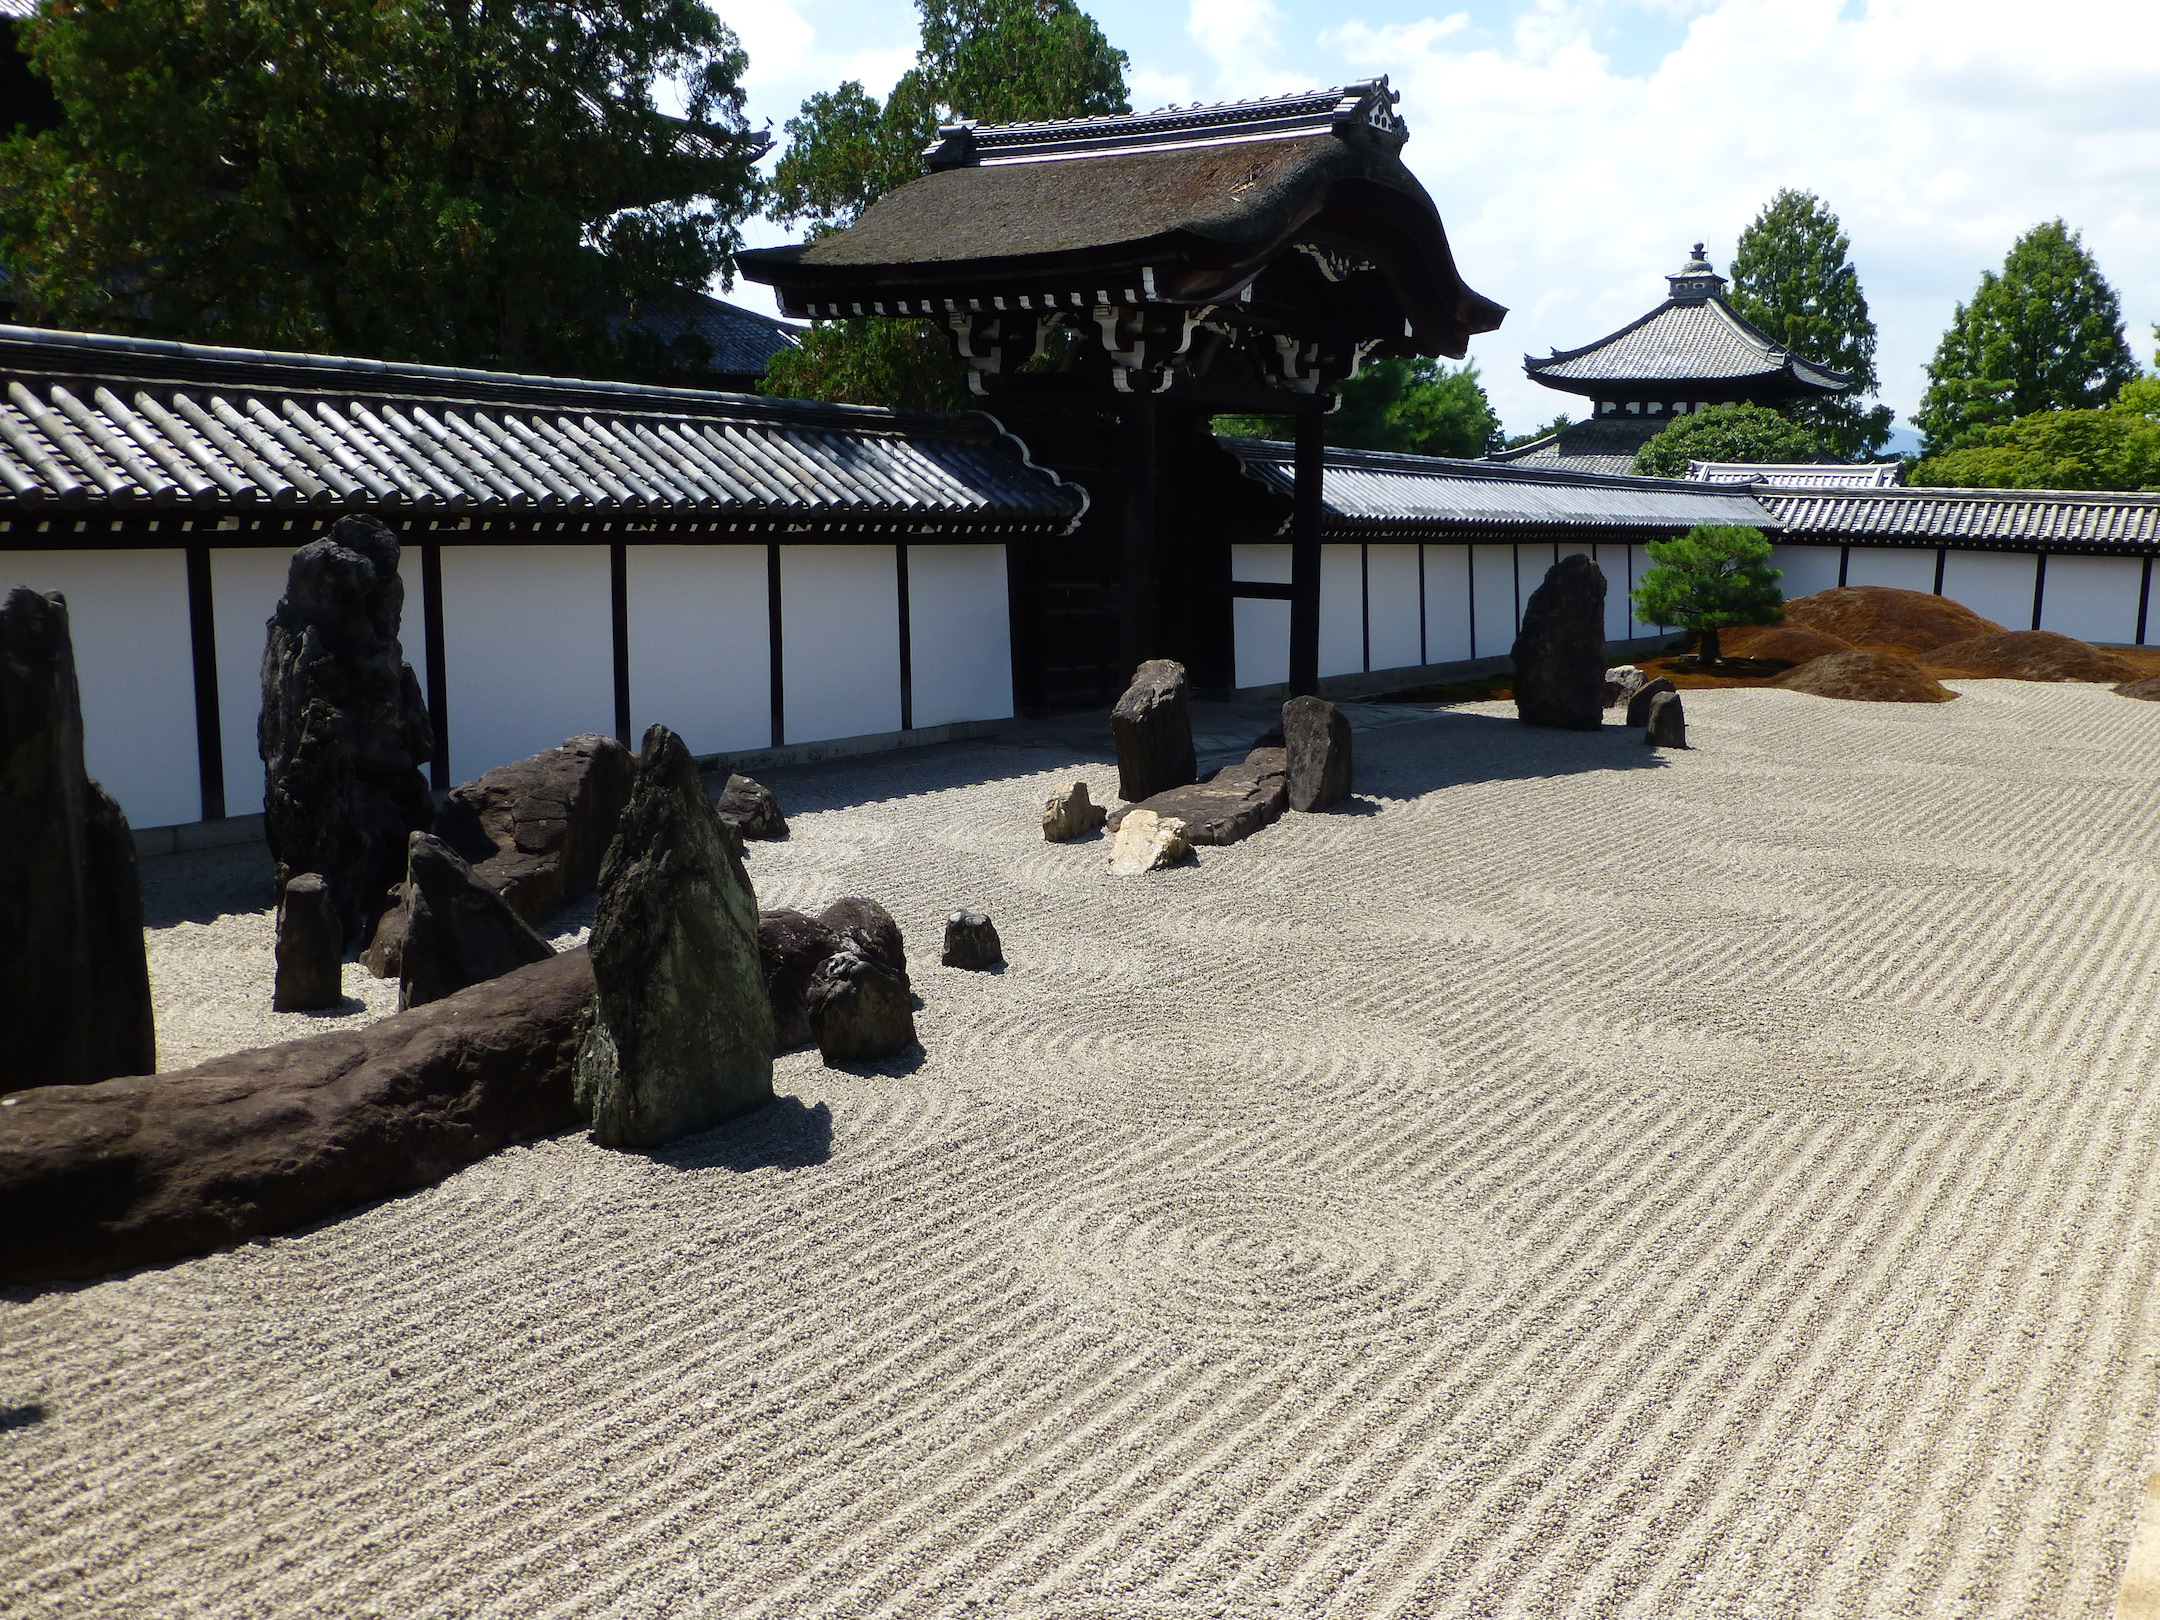
\includegraphics[scale=0.475]
    {figures/jpg/pic06.jpg}
\end{center}
\end{frame}
%-----------------------------------------------------------------------
\section{Scoping}
\begin{frame}[fragile]
\frametitle{Scoping}

\begin{itemize}
\item The \emph{scope} of a variable is the region of code where
  its definition is visible.
\item Scopes are essential for program modularity!
\item There are several mechanisms for introducing scopes and
  defining local variables, including
  \begin{itemize}
  \item Function definitions
  \item $let$ expressions
  \item $where$ clauses
  \end{itemize}
\item Later, we'll see some more.
\end{itemize}

\end{frame}

%-----------------------------------------------------------------------
\subsection{let expressions}

\begin{frame}[fragile]
\frametitle{let expressions}

\begin{itemize}
\item A $let$ expression provides a \emph{local scope}:
  \begin{itemize}
  \item There is a \emph{set of equations} that define some
    variables,
  \item and an \emph{expression} that is evaluated \emph{with those
      variables in scope}.
  \end{itemize}
\item Outside the $let$ expression, the variables defined in the
  equations are \emph{not} in scope.
\end{itemize}

General form:

\begin{verbatim}
let x = exp1
    y = exp2
    z = exp3
in exp
\end{verbatim}

\end{frame}

%-----------------------------------------------------------------------
\begin{frame}[fragile]
\frametitle{Examples of let expressions}

\begin{verbatim}
2 * (let x = 2+2 in x*3) + 1
\end{verbatim}

\begin{verbatim}
let x = 2*3 in (x-1, x+1)
\end{verbatim}

\begin{verbatim}
let x = y+5
    y = 7
in y^2
\end{verbatim}

\end{frame}

%-----------------------------------------------------------------------
\subsection{where clauses}

\begin{frame}[fragile]
\frametitle{where clauses}

\begin{itemize}
\item A $where$ clause is another syntax for introducing local
  definitions.
\item It appears inside an equation (it needs to be indented
  properly to indicate this).
\item It begins with the keyword $where$, followed by one or more
  equations.
\item The right hand side of the top level definition can use the
  variables defined in the equations.
\end{itemize}

\begin{verbatim}
f x = a^2 - b
  where a = x+1
        b = 2*3
\end{verbatim}

\end{frame}

%-----------------------------------------------------------------------
\begin{frame}[fragile]
\frametitle{Example of a where clause}

This example has two three scopes:

\begin{itemize}
\item Inside the body of $f$, the variable $x$ is bound to the argument..
\item Inside the $let$ expression, $a=3$ and $b$ is bound by its
  equation.
\item Inside the right hand side of $b$'s equation, $a=10*x$.
\end{itemize}

\begin{verbatim}
f :: Int -> (Int,Int)
f x =
  let a = 3
      b = a+1
        where a = 10*x
  in (a,b)
\end{verbatim}

\begin{verbatim}
f 5 -- > (3,51)
\end{verbatim}

\end{frame}

%-----------------------------------------------------------------------
\begin{frame}[fragile]
\frametitle{Comparison of $let$ and $where$}

\begin{itemize}
\item Similarities
  \begin{itemize}
  \item Both introduce a local scope.
  \item Both allow any number of equations to be written.
  \item Both allow the equations to be written in any order, and
    variables defined in any equation can be used (``are in scope'')
    in the other equations.
  \end{itemize}
\item Differences
  \begin{itemize}
  \item $let$ expressions are \emph{expressions}; let can be used
    \emph{anywhere} an expression is allowed.
  \item $where$ clauses are \emph{not} expressions; they can be
    used only to provide some local variables for a top level
    equation.
  \end{itemize}
\end{itemize}

\end{frame}

%-----------------------------------------------------------------------
\section{Conditionals}
\begin{frame}[fragile]
\frametitle{Conditionals}

\begin{itemize}
\item We have already seen one form of conditional: the
  if-then-else expression.
\item Two more are now introduced:
  \begin{itemize}
  \item Guarded equations
  \item The $case$ expression
  \end{itemize}
\end{itemize}

\end{frame}

%-----------------------------------------------------------------------
\subsection{Guards}

\begin{frame}[fragile]
\frametitle{Guards}

A common notation in mathematics is to define something with everal
separate values, depending on ``guard conditions''.

\begin{equation}
f_{n} =
\begin{cases}
  n  & \text{if $n$ is even,} \\
  n+1  & \text{if $n$ is odd.} \\
\end{cases}
\end{equation}

Haskell provides a similar notation for defining functions; it's
called \emph{guards}.

\begin{verbatim}
f x
  | predicate1   = exp1 
  | predicate2   = exp2
  | predicate3   = exp3
\end{verbatim}

There can, of course, be any number of guarded equations.

\end{frame}

%-----------------------------------------------------------------------
\begin{frame}[fragile]
\frametitle{Two ways to define absolute value}

You can use an if-then-else expression:

\begin{verbatim}
abs x = if x<0 then (-x) else x
\end{verbatim}

Alternatively, guarded equations correspond to traditional
mathematical style.

\begin{verbatim}
abs x
  | x<0        = -x
  | otherwise  = x
\end{verbatim}

\end{frame}

%-----------------------------------------------------------------------
\begin{frame}[fragile]
\frametitle{Another example of guards}

Guards are clearer than if-then-else if there are three or more
conditions.

\begin{verbatim}
data Sgn = Neg $ Zero $ Pos
  deriving (Read, Show)
\end{verbatim}

This function takes an $Int$ and gives its $Sgn$:

\begin{verbatim}
sgn :: Int -> Sgn
sgn x
  | x<0    = Neg
  | x==0   = Zero
  | x>0    = Pos
\end{verbatim}

\end{frame}

%-----------------------------------------------------------------------
\subsection{Constructors and case expressions}

\begin{frame}[fragile]
\frametitle{Constructors are functions that construct data}

\begin{itemize}
\item An algebraic data type has one or more \emph{constructors}.
\item You can think of a constructor in several ways:
  \begin{itemize}
  \item It is a function (of zero or more arguments) that builds a
    piece of data.
  \item It serves as a tag that identifies which kind of data this
    is, from the set of alternatives.
  \end{itemize}
\end{itemize}

\begin{verbatim}
data Tree a
  = Leaf a
  | Node a (Tree a) (Tree a)
\end{verbatim}

The constructors are:

\begin{verbatim}
Leaf :: a -> Tree a
Node :: a -> Tree a -> Tree a -> Tree a
\end{verbatim}

\end{frame}

%-----------------------------------------------------------------------
\begin{frame}[fragile]
\frametitle{Constructors indicate which kind of data}

The representation of $x$ indicates that it's a $Leaf$, and the
representation of $y$ indicates that it's a $Node$:

\begin{verbatim}
p, q :: Tree String
p = Leaf "cat"
q = Node "animals" x (Leaf "dog")
\end{verbatim}

\end{frame}

%-----------------------------------------------------------------------
\begin{frame}[fragile]
\frametitle{Case expressions}

\begin{itemize}
\item A data value with an algebraic data type may have
  several different forms.
  \begin{itemize}
  \item A value of type $Tree a$ must be either a $Leaf$ or a
    $Node$.
  \end{itemize}
\item Therefore to process such a value we need several different
  pieces of code, one for each possible form.
\item The $case$ expression examines the constructor, and chooses
  the corresponding piece of code.
\end{itemize}

\begin{verbatim}
f :: Tree String -> String
f x =
  case x of
    Leaf s -> "Leaf " ++ s
    Node n left right -> "Node " ++ s

f p -- > "Leaf cat"
f q -- > "Node dog"
\end{verbatim}

\end{frame}

%-----------------------------------------------------------------------
\begin{frame}[fragile]
\frametitle{Case expressions with a Bool}

\begin{verbatim}
data Bool
  = False
  | True
\end{verbatim}

\begin{verbatim}
case b of
  False -> exp1
  True  -> exp2
\end{verbatim}

\end{frame}

%-----------------------------------------------------------------------
\begin{frame}[fragile]
\frametitle{Evaluation of a Bool case}

\begin{verbatim}
f :: Int -> Int
f x =
  case x<0 of
    False -> x
    True  -> -x
  \end{verbatim}

\begin{verbatim}
  f (-3)
-- >
  case (-3)<0 of
    False -> (-3)
    True  -> -(-3)
-- >
  case True of
    False -> (-3)
    True  -> -(-3)
-- > -(-3) -- > 3
\end{verbatim}

\end{frame}

%-----------------------------------------------------------------------
\begin{frame}[fragile]
\frametitle{Implementation of if-then-else}

\begin{verbatim}
if b then e1 else e2
\end{verbatim}

is syntactic sugar for

\begin{verbatim}
case b of
  True  -> e1
  False -> e2
\end{verbatim}

``Syntactic sugar'' means that the language allows you to write
if-then-else expressions, but they are translated into the $case$
expression.

The basic language, without the syntactic sugar, is called the
\emph{core language}.

\end{frame}

%-----------------------------------------------------------------------
\section{Maybe}

\begin{frame}[fragile]
\frametitle{Maybe}

\begin{itemize}
\item A fact of life in programming is that many computations might
  fail.
\item Programmers in imperative languages are often sloppy with
  such computations --- that's one reason that software sometimes
  crashes.
\item Haskell provides several mechanisms for handling computations
  that might fail.
\item The first --- and simplest --- is $Maybe$.
\item Later we'll see several more, and discuss when each method is
  most appropriate.
\end{itemize}

\end{frame}

%-----------------------------------------------------------------------
\begin{frame}[fragile]
\frametitle{Computations that might fail}

\begin{itemize}
\item Often you perform a computation that would normally succeed,
  but it might occasionally fail.
  \begin{itemize}
  \item A division where the divisor might possibly be 0
  \item Applying $head$ or $tail$ to a list, where the list might
    possibly be $[]$
  \item Reading the contents of a file, where the file might not exist.
  \end{itemize}
\item What we need is a way to report whether a computation has
  succeeded, so the rest of the program can either
  \begin{itemize}
  \item get on with the successful computation, or
  \item cope with the failure.
  \end{itemize}
\end{itemize}

\end{frame}

%-----------------------------------------------------------------------
\begin{frame}[fragile]
\frametitle{$Maybe$}

\begin{itemize}
\item $Maybe a$ is an algebraic data type that represents the
  result of an attempt to compute a value of type $a$.
\item If the computation fails, we get nothing.
\item If it succeeds, we just get a value of type $a$.
\end{itemize}

\begin{verbatim}
data Maybe a
  = Nothing
  | Just a
\end{verbatim}

The point is that the constructors \emph{tag the result, so we can
  tell whether we have a result}.

\end{frame}

%-----------------------------------------------------------------------
\begin{frame}[fragile]
\frametitle{Safe division}

\begin{itemize}
\item If we divide with $div$, there is an error if the divisor is 0.
\item The error will abort the program (although it's possible to
  catch such errors).
\item We can \emph{guarantee} that a division will \emph{never}
  abort the program by using a ``safe division'' that uses $Maybe$.
\end{itemize}

\begin{verbatim}
safeDiv :: Double -> Double -> Maybe Double
safeDiv x y
  | y==0       = Nothing
  | otherwise  = x / y
\end{verbatim}

\end{frame}

%-----------------------------------------------------------------------
\begin{frame}[fragile]
\frametitle{Handling the result of a $Maybe$}

\begin{itemize}
\item Now, when we use $safeDiv$, we need to check the result to
  see whether it's $Nothing$.
\item This is done with a $case$ expression.
\end{itemize}

Example: compute $(a/b)*c$ safely.

\begin{verbatim}
f :: Double -> Double -> Double -> Maybe Double
f a b c =
  case a `safeDiv` b of
    Just q -> Just q*c
    Nothing -> Nothing
  \end{verbatim}

Sometimes, you can handle $Nothing$ with a suitable default value,
so you don't need to return a $Maybe$ type.

\end{frame}

%-----------------------------------------------------------------------
\begin{frame}[fragile]
\frametitle{Discussion of $Maybe$}

\begin{itemize}
\item $Maybe$ provides a way to indicate success or failure, along
  with a result.
\item C also provides a similar mechanism: most standard library
  ``functions'' return a \emph{return code}; 0 indicates ``ok'' and
  non-zero indicates an error.
\item Good practice in C is to check the return code \emph{every time}.
\item Then you need to do something sensible if the return code
  indicates an error.
\item In the real world, few programmers actually do this!  That's
  one of the reasons software sometimes crashes.
\item What about Haskell?
  \begin{itemize}
  \item The $Maybe$ type does \emph{not} solve the hassle of
    deciding what to do if there's an error.
  \item But the great advantage of $Maybe$ is that the typechecker
    \emph{guarantees} that your code will check the result of the
    computation with a $case$ expression.
  \item This helps make code more robust.
  \end{itemize}
\end{itemize}

\end{frame}

%-----------------------------------------------------------------------
\begin{frame}[fragile]
\frametitle{Propagation of $Maybe$}

\begin{itemize}
\item So, you've decided to program robustly and use $Maybe$.
\item It's a bit tedious!  You keep having to write $case$
  expressions to propagate $Nothing$ in the event of an error.
\item What a bore!
\item There must be a better way!
\item \emph{To be continued$\ldots$}

\end{itemize}

\end{frame}

%-----------------------------------------------------------------------
\section{Documentation}

\begin{frame}[fragile]
\frametitle{Documentation}

\begin{itemize}
\item Haskell is fully documented, including
  \begin{itemize}
  \item Language reference manual
  \item Standard Prelude
  \item Additional standard libraries
  \item Packages you can install
  \item Related tools
  \item Tutorials and wiki
  \end{itemize}
\end{itemize}

See the Moodle page for links.

{\redtext Visit the link to the Standard Prelude, and look it over.}

\end{frame}

\end{document}
